\documentclass[12pt]{article}
\usepackage{geometry}                % See geometry.pdf to learn the layout options. There are lots.
\geometry{letterpaper}                   % ... or a4paper or a5paper or ... 
%\geometry{landscape}                % Activate for for rotated page geometry
\usepackage[parfill]{parskip}    % Activate to begin paragraphs with an empty line rather than an indent
\usepackage{daves,fancyhdr,natbib,graphicx,dcolumn,amsmath,lastpage,url}
\usepackage{amsmath,amssymb,epstopdf,longtable}
\usepackage[final]{pdfpages}
\DeclareGraphicsRule{.tif}{png}{.png}{`convert #1 `dirname #1`/`basename #1 .tif`.png}
\pagestyle{fancy}
\lhead{CE 3354 -- Engineering Hydrology}
\rhead{FALL 2024}
\lfoot{ES1}
\cfoot{}
\rfoot{Page \thepage\ of \pageref{LastPage}}
\renewcommand\headrulewidth{0pt}



\begin{document}
\begin{center}
{\textbf{{ CE 3354 Engineering Hydrology} \\ {Exercise Set 1}}}
\end{center}

\section*{\small{Exercises}}
\begin{enumerate}\item Using the internet, textbook(s), and the on-line reading collection define the following (in a sentance or two); please cite your references (URL is sufficient): 
 \begin{enumerate}
 \item Alluvium 
 \item Bankfull Discharge
 \item Best Management Practice
 \item Drainage Divide 
 \item Evaporation 
 \item Evapotranspiration 
 \item Precipitation 
 \item Flow Duration Curve
 \item Flood Frequency Curve
 \item Watershed 
 \item Catchment
 \end{enumerate}

%\item Download and read ``The Underground Subject" Read the pamphlet then prepare answers to the following questions:  What is an aquifer?  In Texas, what is a major aquifer?  In the Lubbock area what kinds of aquifers are present?  Sketch a water table aquifer; label the relevant features.  Sketch a confined aquifer; label the relevant features.  What is the upper boundary for aquifer flow in a confined aquifer? \footnote{The pamphlet is obsolete with regards to ownership - water law in Texas has changed substantially since the pamphlet was printed.}

\item Assuming that all water in the oceans is involved in the hydrologic cycle, estimate the average residence time of ocean water. [Problem 1.1.1 in Chow, Maidment, and Mays]

\item Assuming that all surface runoff to the oceans comes from rivers, estimate the average residence time of water in rivers. [Problem 1.1.2 in Chow, Maidment, and Mays]

\item The equation $k\frac{dQ}{dt} + Q(t) = I(t)$ has been used to describe the response of streamflow to a constant rate of precipitation continuing indefinitely on a watershed.  For this problem, let $I(t) =1$ for $t>0$ and $Q(t) =0$ for $t=0$. Plot values of $I(t)$ and $Q(t)$ over a 10-hour period if $k=2$.  [Problem 1.3.2 in in Chow, Maidment, and Mays]\footnote{You will need to solve the differential equation}

\clearpage
 
 
%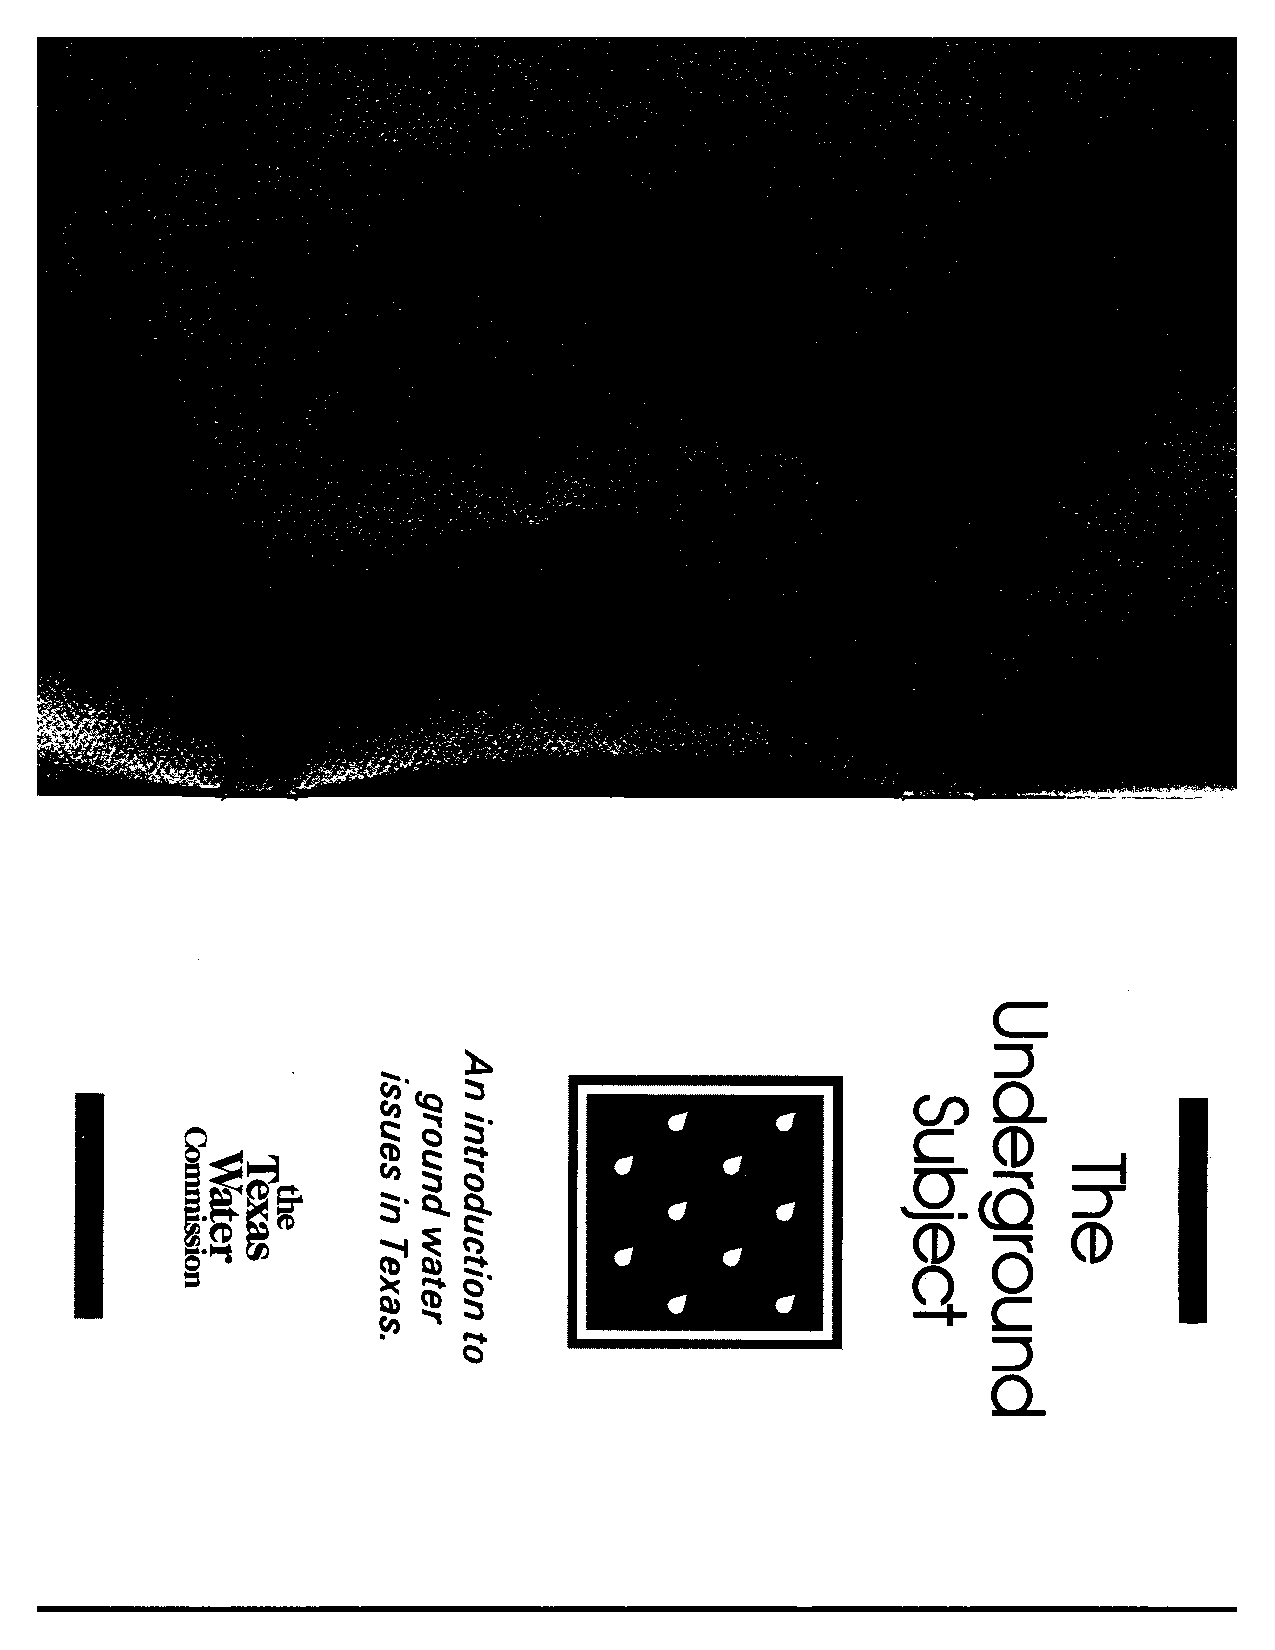
\includepdf[pages={-}]{./TWC_8905.pdf}
 
\item Figure \ref{fig:farmland} is a schematic of a 600-hectare farm; the land receives annual rainfall of 2500 mm.  There is a river flowing through the farm land with inflow rate of 5 m$^3$/s and outflow rate of 4m$^3$/s.  The annual water storage in the farm land increases by 2.5$\times$10$^6$m$^3$.  Using the water budget concept, estimate the annual evaporation amount in millimeters.\footnote{1 hectare = 10,000 m$^2$}

\begin{figure}[h!] %  figure placement: here, top, bottom, or page
   \centering
   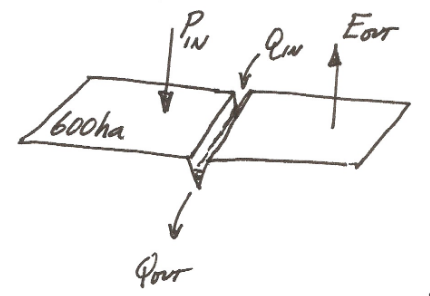
\includegraphics[width=4in]{farmland.png} 
   \caption{Schematic of Farmland}
   \label{fig:farmland}
\end{figure}

\item A reservoir has a surface area of 690 acres.  Figure \ref{fig:reservoir} shows the monthly inflow of surface water, outflows as releases from the reservoir via the spillway, direct precipitation into the reservoir, and evaporation from the reservoir.  The reservoir water surface elevation was 701.0 feet on January 1.  Determine the reservoir water surface elevation at the end of each month (i.e. complete the table)

\begin{figure}[h!] %  figure placement: here, top, bottom, or page
   \centering
   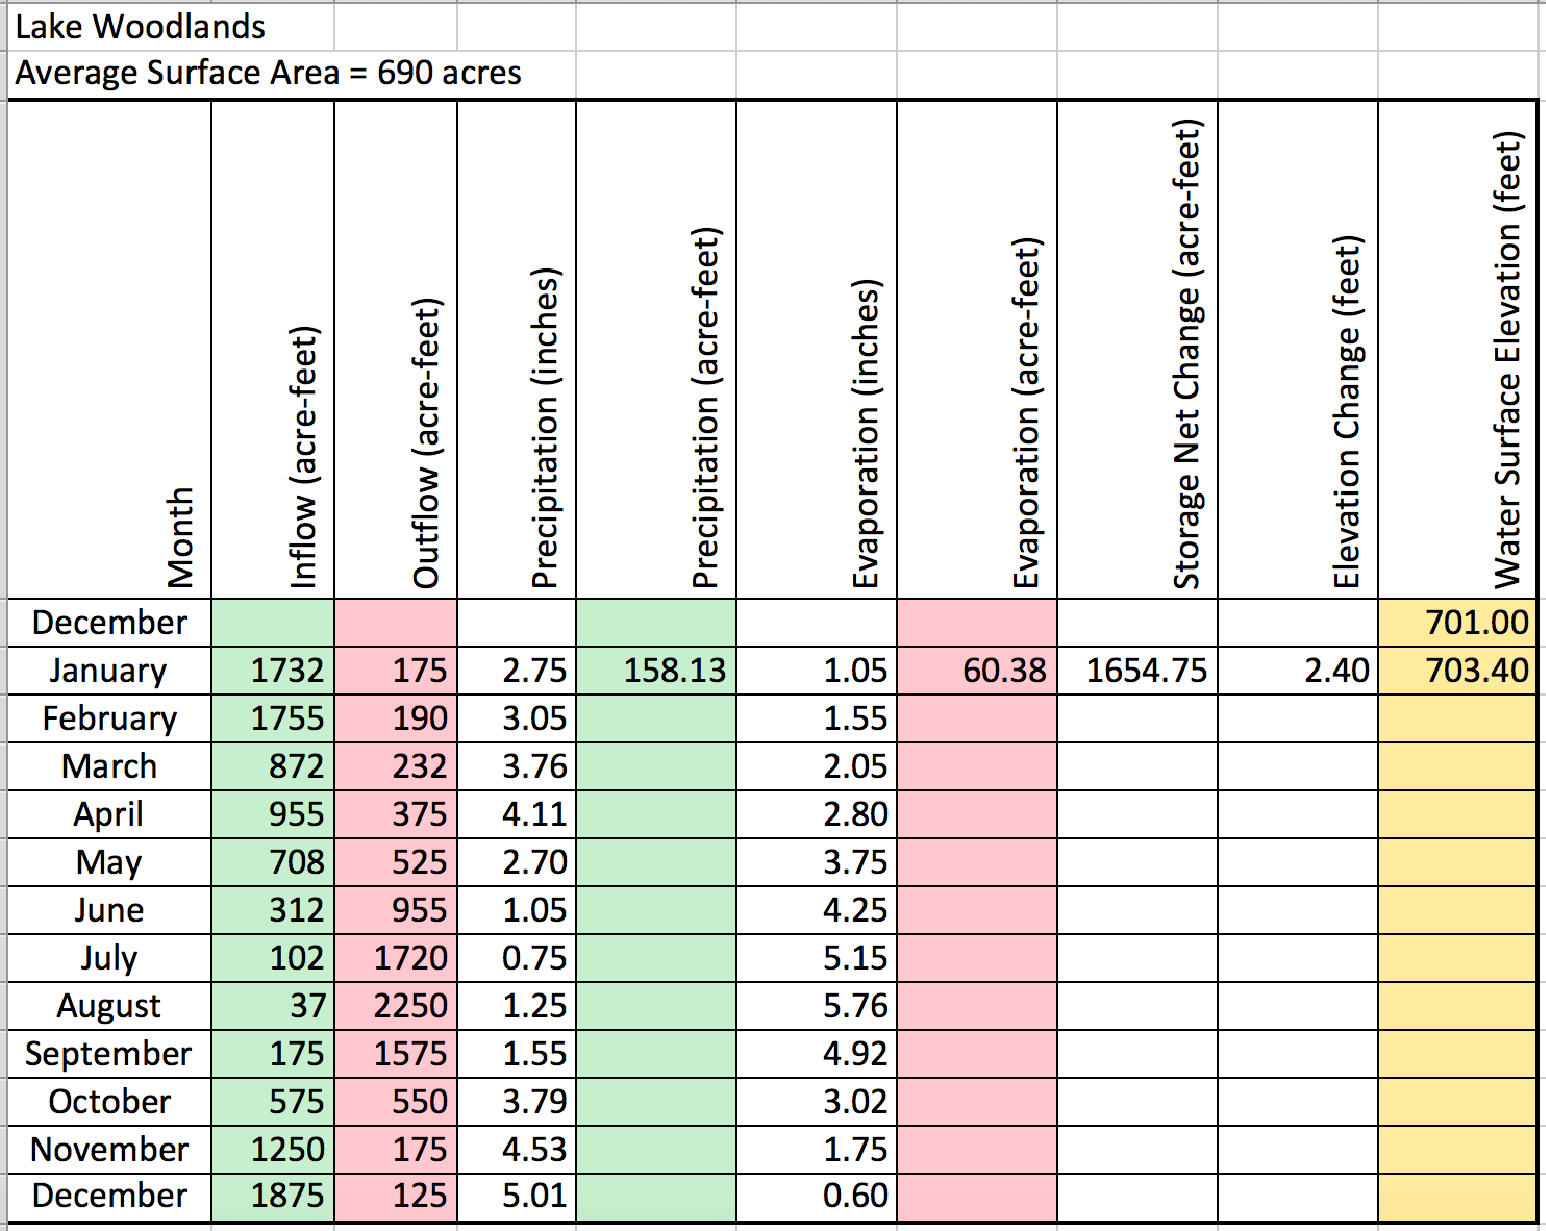
\includegraphics[width=6in]{Reservior.pdf} 
   \caption{Tabular Water Budget Values}
   \label{fig:reservoir}
\end{figure}



\end{enumerate}


\end{document}  